\begin{center}	
\textbf{BOLETÍN DE EJERCICIOS 3}
\end{center}

\vspace{2cm}

\textbf{Diagnóstico y retos de la economía Española:\\
	Tasa de actividad femenina.}\\\\

    \begin{center}
	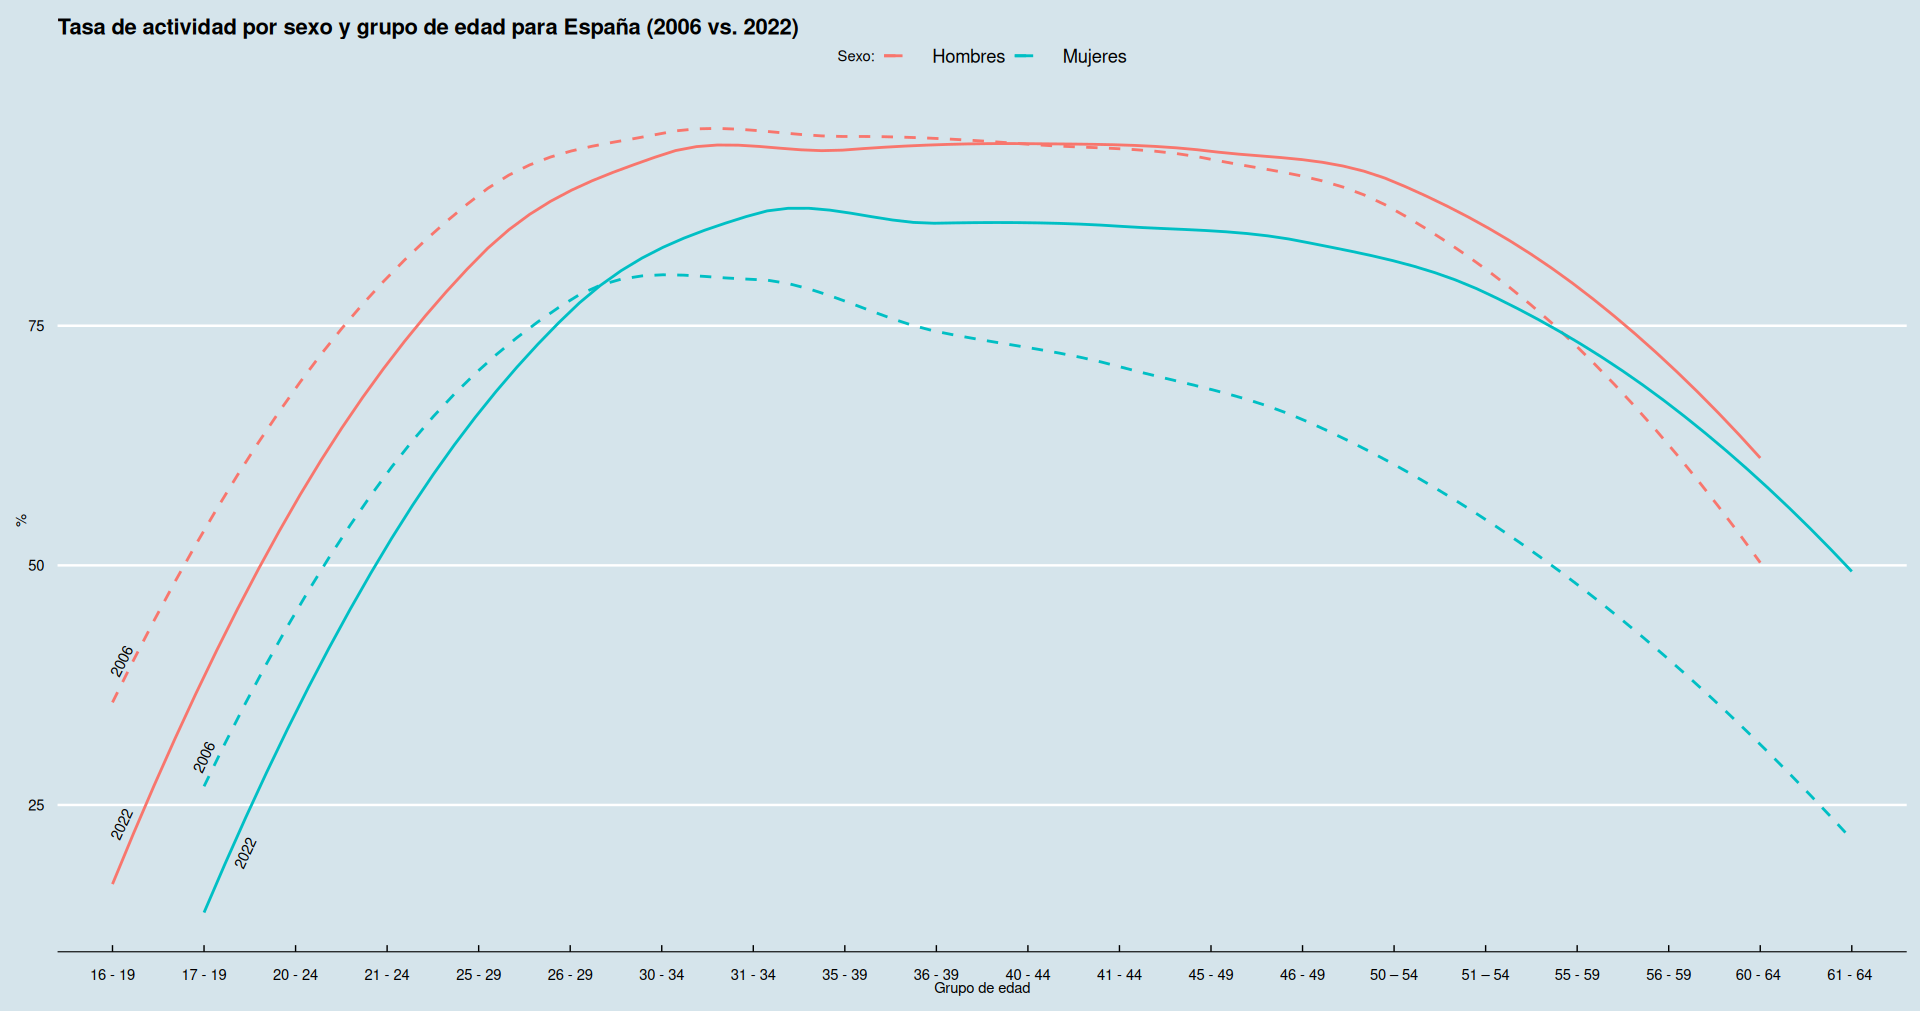
\includegraphics[scale=.32]{image/b3ej1e.png}
    \end{center}
    \vspace{.5cm}


En el grupo de edad de 16 a 19 años, se registra una disminución significativa en la tasa de actividad femenina en el año 2022 en comparación con 2006. Esto puede indicar cambios en la estructura educativa y la preferencia por continuar estudios en lugar de incorporarse tempranamente al mercado laboral.\\

En contraste, en los grupos de edad de 20 a 54 años, se evidencia un incremento notable en la tasa de actividad femenina en 2022 en comparación con 2006. Esto sugiere un mayor nivel de participación laboral de las mujeres en estas edades, reflejando avances en la igualdad de género y en la promoción de la incorporación de la mujer al campo laboral.\\

En los grupos de edad más avanzada, a partir de los 55 años, se aprecia una disminución en la tasa de actividad femenina en 2022 en comparación con 2006. Específicamente, en los grupos de edad de 55 a 59 años y 60 años en adelante, se registra una reducción en la participación laboral de las mujeres. Esto puede estar relacionado con factores como la jubilación anticipada o la falta de oportunidades laborales para mujeres mayores.\\

En resumen, al comparar los datos de la tasa de actividad femenina en España entre los años 2006 y 2022, se observa un incremento en la participación laboral de las mujeres en los grupos de edad de 20 a 54 años, lo que indica avances en la igualdad de género y en la incorporación de la mujer al mercado laboral. Sin embargo, se requiere una mayor atención y políticas específicas para abordar la disminución en la tasa de actividad femenina en los grupos de edad más jóvenes (16-19 años) y en los grupos de edad más avanzada (55 años en adelante).\\\\



\textbf{Diagnóstico y retos de la economía Alemana:\\
	Tasa de participación en la fuerza laboral femenina.}\\\\

    \begin{center}
	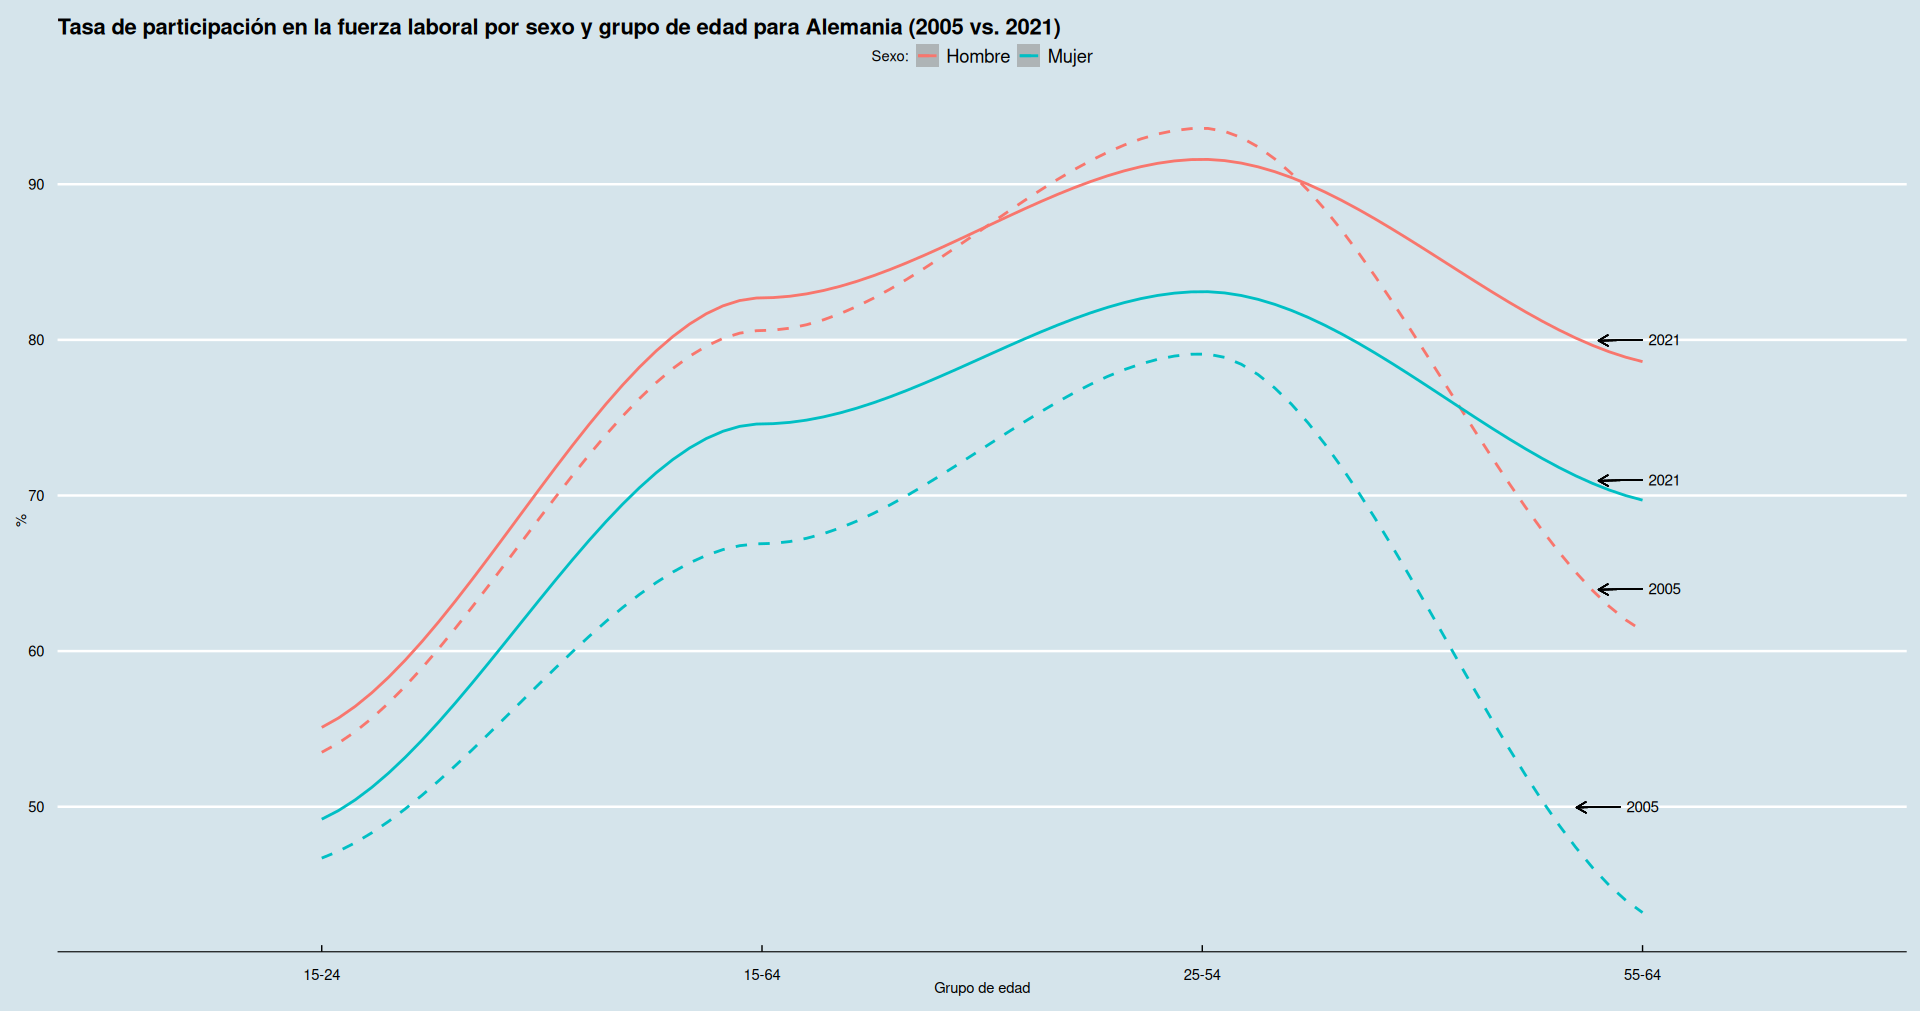
\includegraphics[scale=.32]{image/b3ej1.png}
    \end{center}
    \vspace{.5cm}

Comparando los datos para el grupo de mujeres de 15-24 años, observamos que la Tasa de participación en la fuerza laboral en 2005 era del 46.7\%, mientras que en 2021 aumentó ligeramente a 49.2\%. Esto indica un ligero aumento en la participación laboral de las mujeres jóvenes en ese período en Alemania.\\

En el grupo de mujeres de 15-64 años, vemos un aumento en la tasa de actividad de 66.9\% en 2005 a 74.6\% en 2021. Esto indica que más mujeres en este rango de edad están participando en el mercado laboral en comparación con 2005.\\

Al analizar el grupo de mujeres de 25-54 años, observamos un aumento en la Tasa de participación en la fuerza laboral del 79.1\% en 2005 al 83.1\% en 2021. Este incremento sugiere una mayor participación laboral de las mujeres en edad media, lo cual es una tendencia positiva en términos de igualdad de género y empoderamiento económico.\\

En el grupo de mujeres de 55-64 años, la Tasa de participación en la fuerza laboral aumentó significativamente del 43.2\% en 2005 al 69.7\% en 2021. Este aumento indica una mejora notable en la participación laboral de las mujeres mayores en Alemania.\\

Estas conclusiones muestran una tendencia positiva en cuanto a la participación laboral de las mujeres en Alemania en distintas etapas de la vida, lo cual es un indicador relevante en términos de igualdad de género y desarrollo económico.\\\\


\newpage

\textbf{Diagnosis del mercado de trabajo (1)}

    \begin{center}
	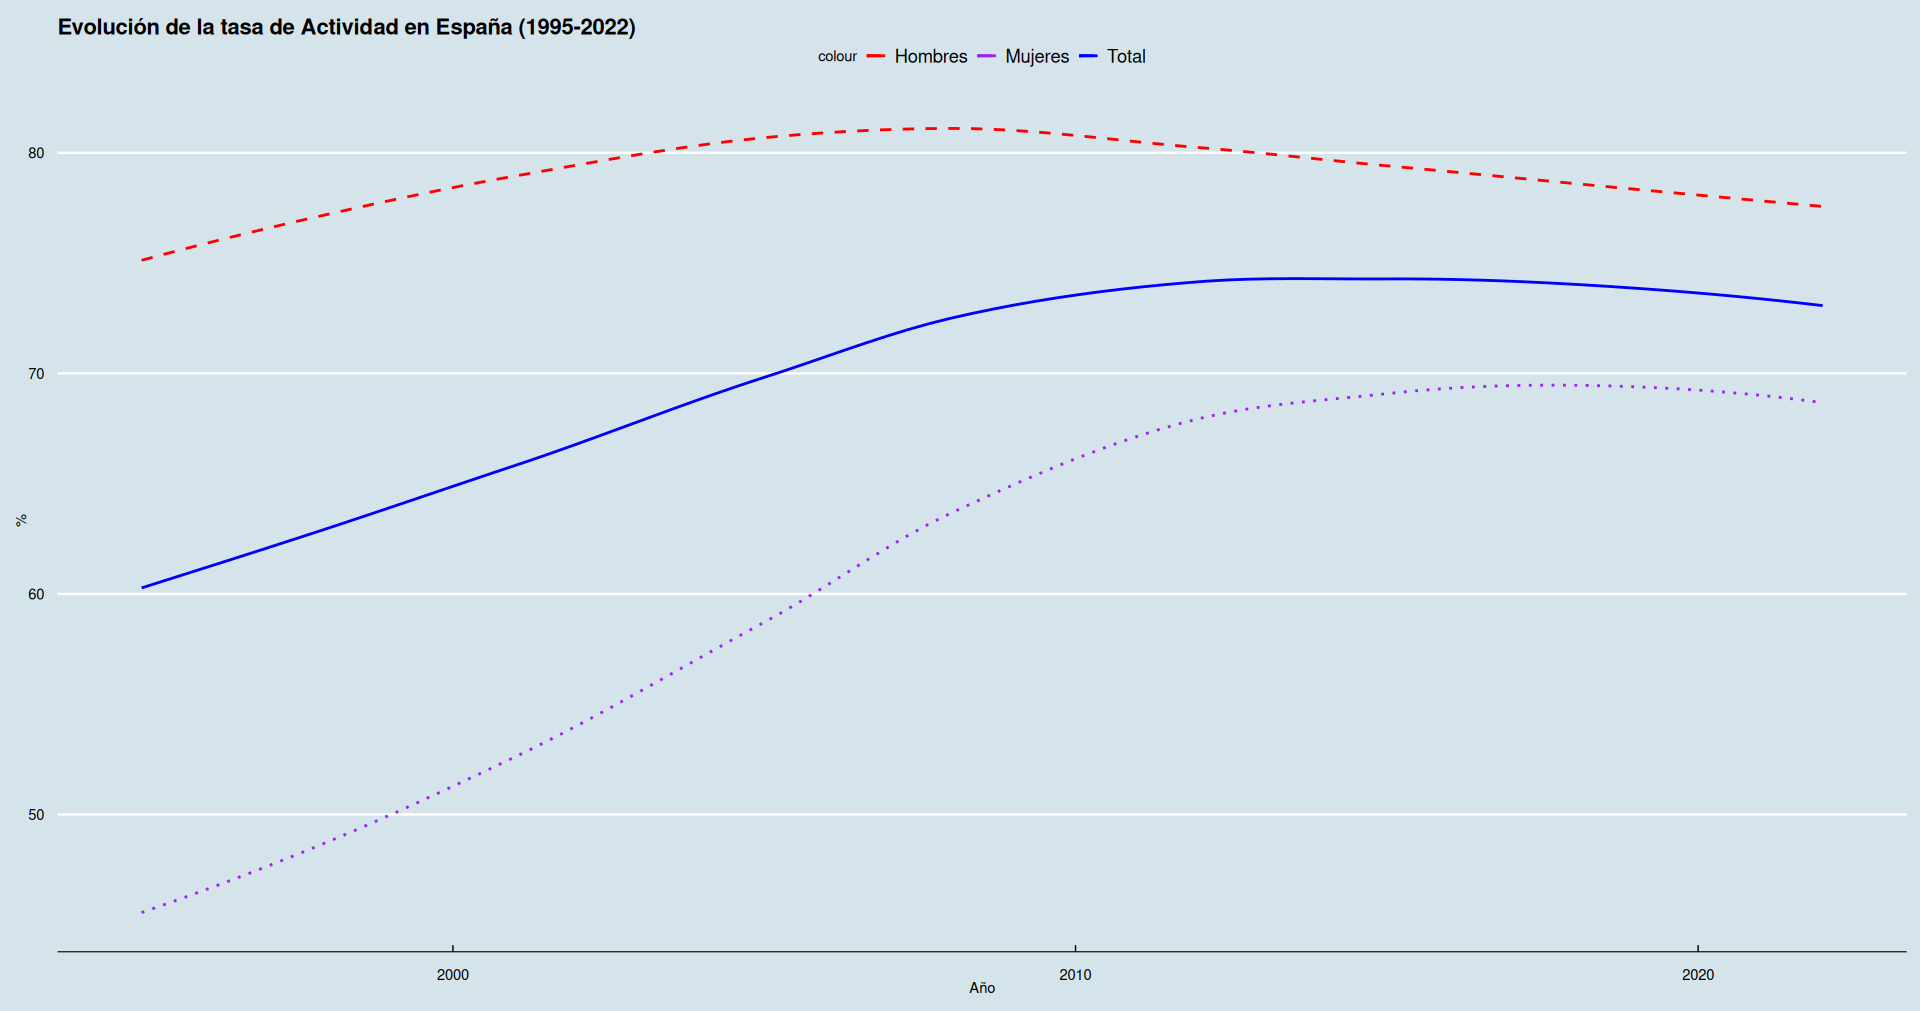
\includegraphics[scale=.32]{image/b3ej2e.png}
    \end{center}
    \vspace{.5cm}

    Al analizar la evolución de la tasa de actividad femenina en comparación con la masculina en España, se pueden destacar dos conclusiones relevantes. En primer lugar, se observa un aumento constante en la tasa de actividad femenina a lo largo del período analizado. Esto indica una creciente participación de las mujeres en el mercado laboral.\\

No obstante, a pesar de este progreso, persiste una brecha de género en términos de la tasa de actividad. A lo largo de los años, la tasa de actividad masculina se mantiene consistentemente por encima de la tasa de actividad femenina. Aunque se puede apreciar una reducción en esta brecha a lo largo del tiempo, es evidente que aún existen disparidades significativas entre hombres y mujeres en cuanto a su participación en el mercado laboral.


    \begin{center}
	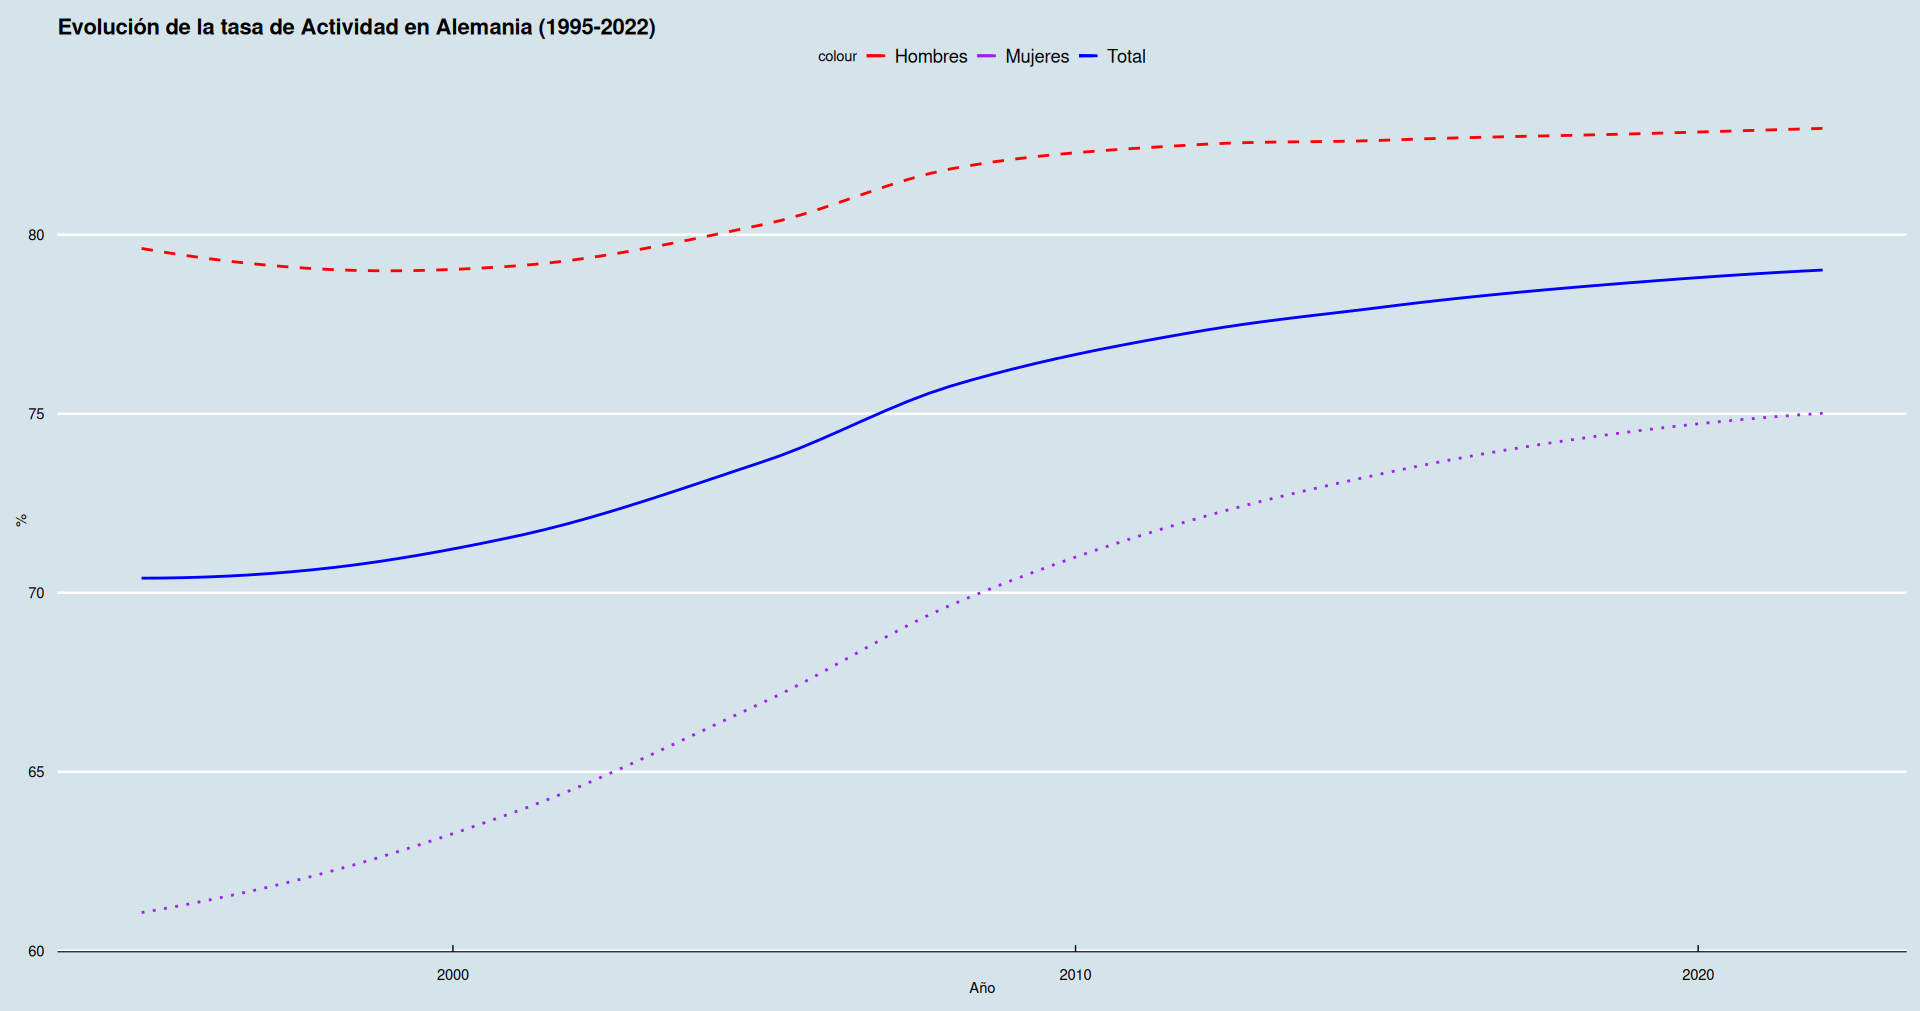
\includegraphics[scale=.32]{image/b3ej2a.png}
    \end{center}
    \vspace{.5cm}

    Al analizar la evolución de la tasa de actividad femenina en relación con la masculina en Alemania, se pueden extraer dos conclusiones relevantes. Primero, se observa una persistente brecha de género en la participación laboral. A lo largo de los años, la tasa de actividad masculina ha sido consistentemente más alta que la tasa de actividad femenina. En el año 2022, la tasa de actividad femenina se situó en aproximadamente un 75.4\%, mientras que la tasa de actividad masculina alcanzó alrededor del 83.4\%. Estos datos indican una disparidad en la participación laboral entre hombres y mujeres en Alemania.\\

Sin embargo, se destaca una tendencia de convergencia a lo largo del tiempo. A pesar de la brecha de género, se ha registrado un aumento gradual en la tasa de actividad femenina, lo que sugiere un mayor equilibrio en términos de oportunidades laborales y roles de género. Esta tendencia refleja la importancia de las políticas y medidas implementadas para promover la igualdad de género en el ámbito laboral en Alemania.

'\newpage

\textbf{Diagnostico del mercado de trabajo (2)}

    \begin{center}
	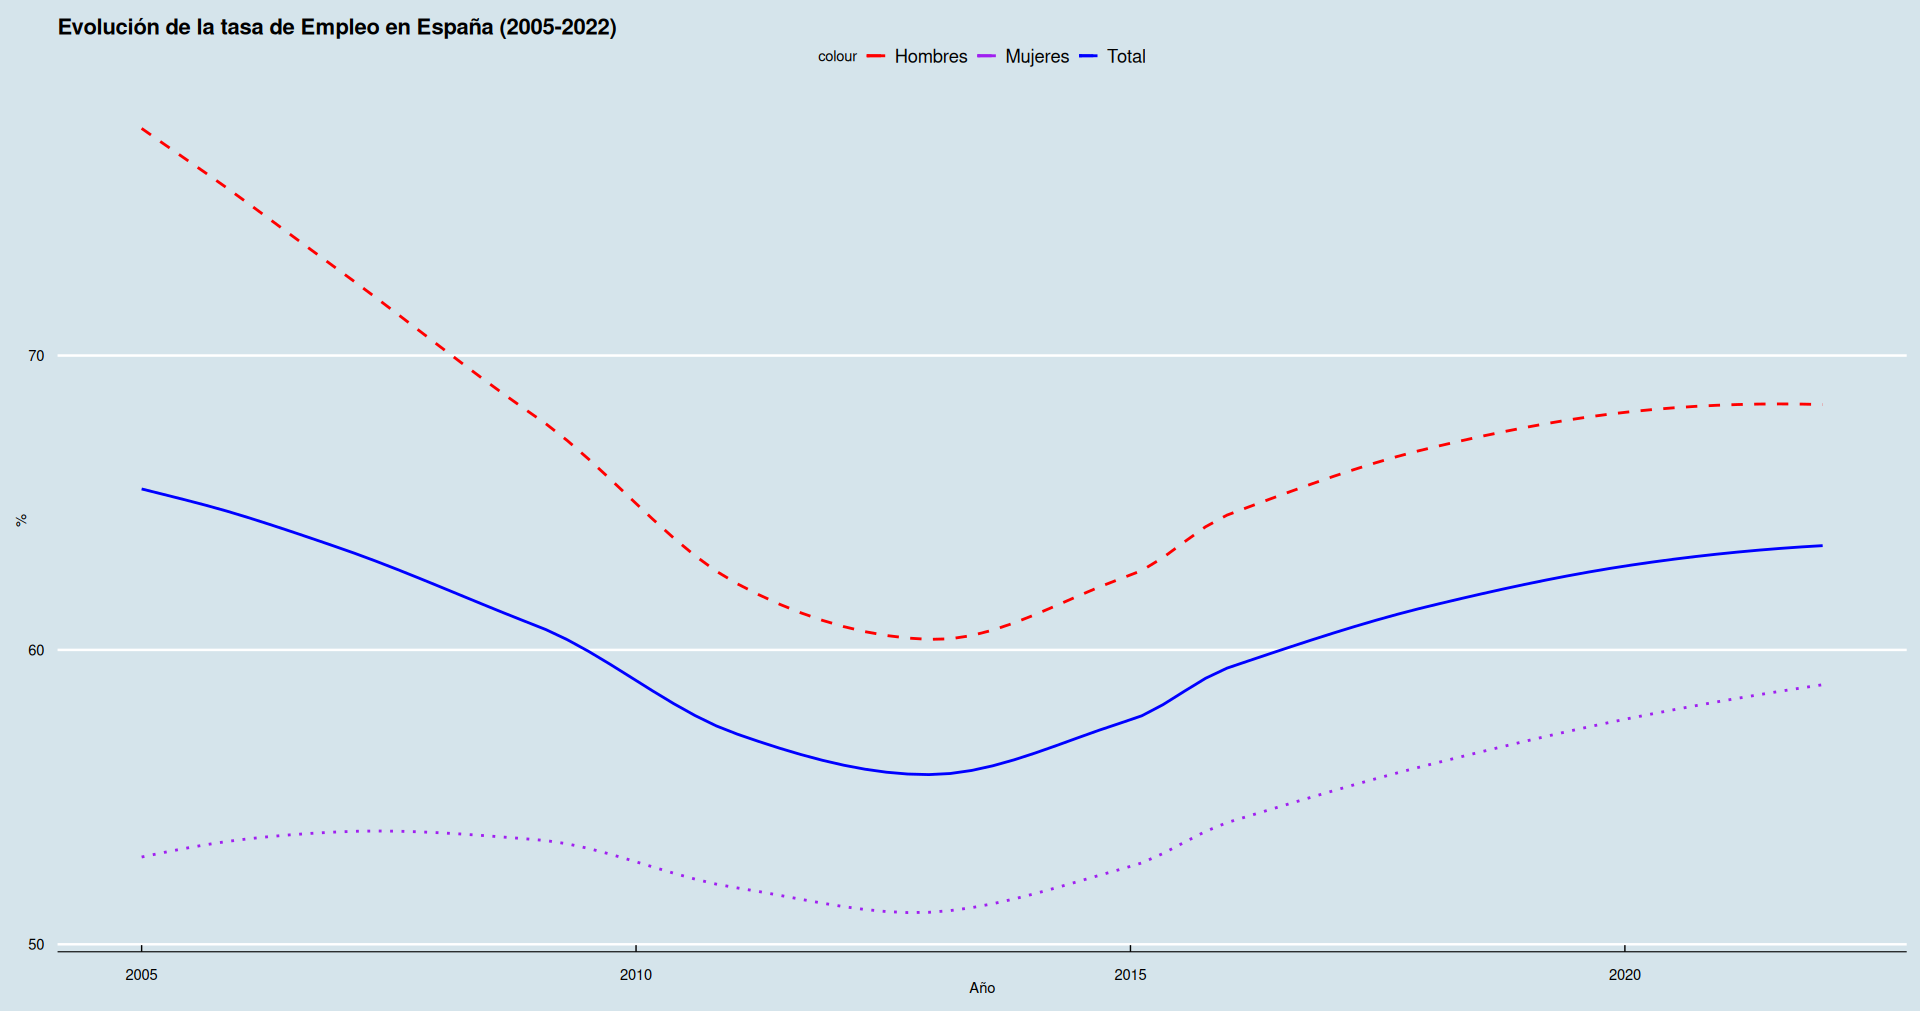
\includegraphics[scale=.32]{image/b3ej3e.png}
    \end{center}
    \vspace{.5cm}
    Durante el período de 2005 a 2022, se observa una evolución significativa en la tasa de empleo femenino en España en comparación con la tasa de empleo masculino y la tasa de empleo total. En general, se evidencia un incremento progresivo de la tasa de empleo femenino, lo cual indica una mayor participación de las mujeres en el mercado laboral español a lo largo del tiempo. A pesar de este avance, persiste una brecha de género en el mercado laboral, ya que la tasa de empleo masculino ha sido consistentemente más alta que la tasa de empleo femenino en todos los años considerados.\\\\

    \begin{center}
	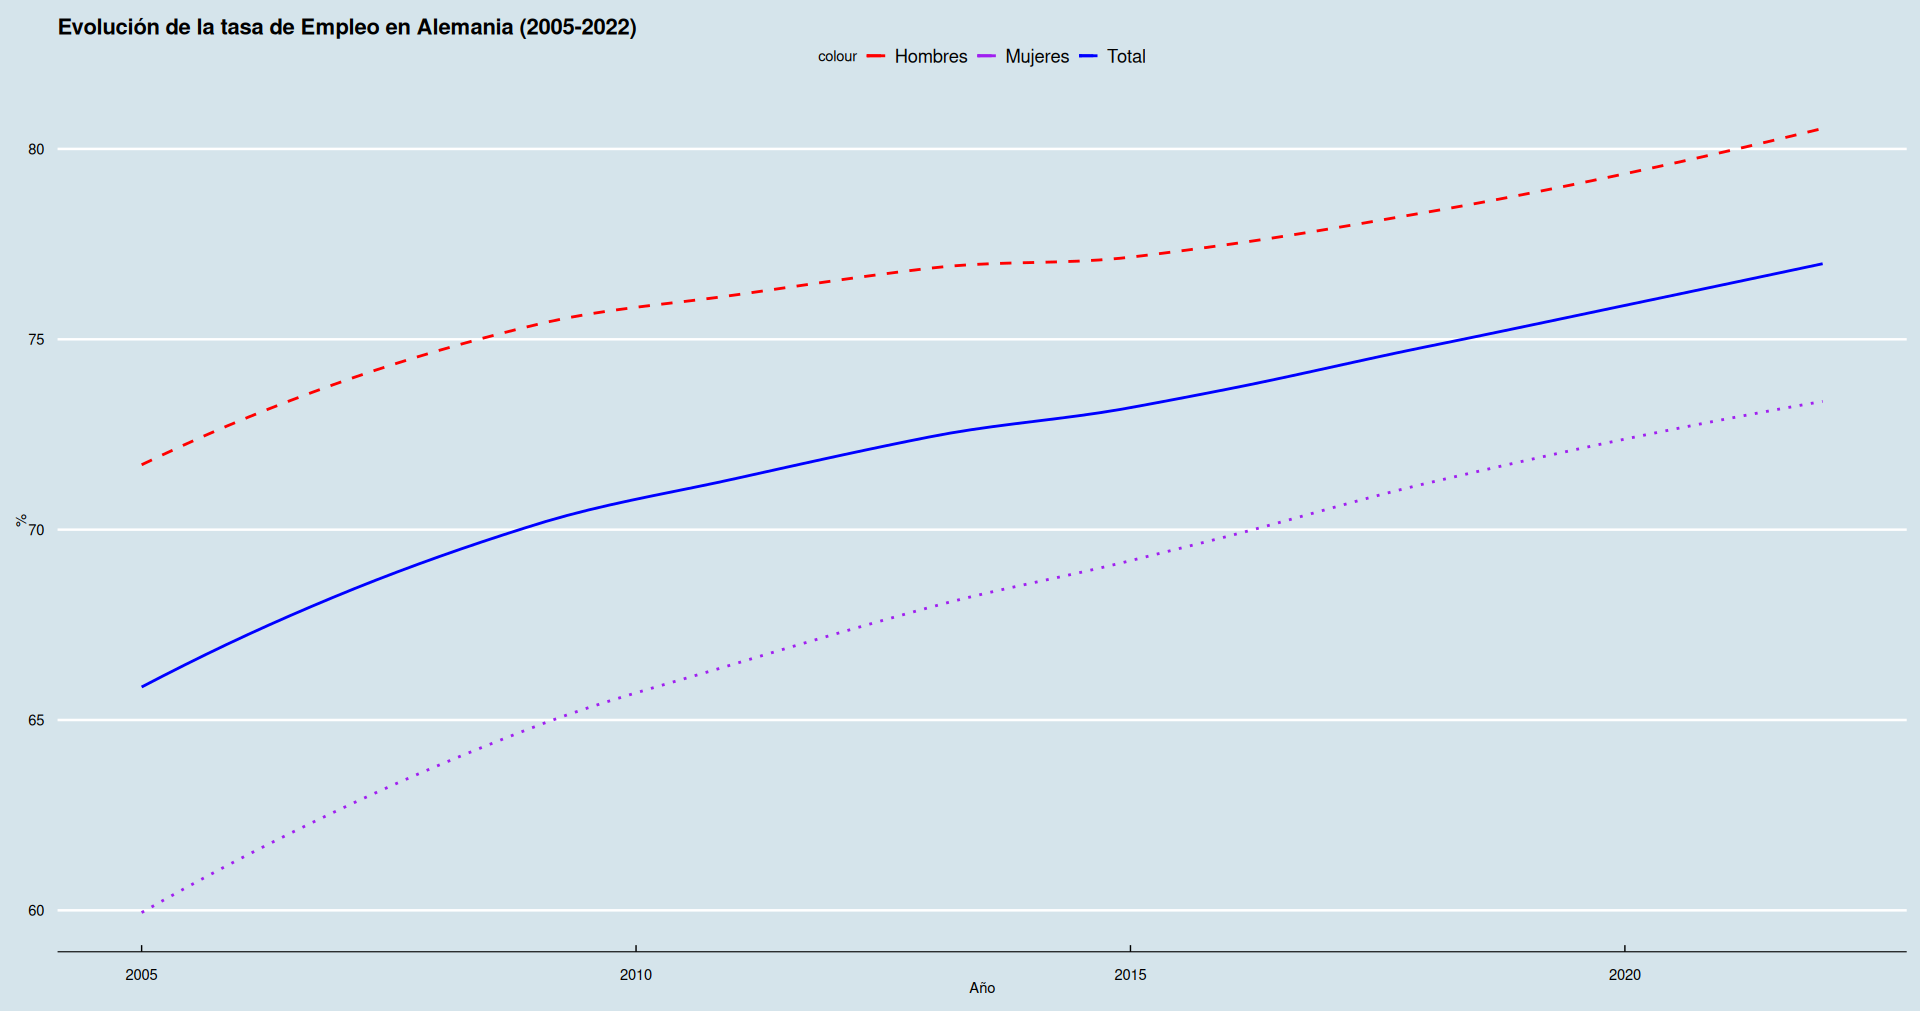
\includegraphics[scale=.32]{image/b3ej3a.png}
    \end{center}
    \vspace{.5cm}

    Durante el periodo analizado de 2005 a 2022, se pueden extraer dos conclusiones relevantes sobre la evolución de la tasa de empleo de las mujeres en Alemania en comparación con la tasa de empleo de los hombres y la tasa de empleo total. En primer lugar, se observa un incremento constante en la tasa de empleo de las mujeres, lo que indica una mayor participación de las mujeres en el mercado laboral alemán a lo largo de los años. Este crecimiento sostenido refleja los esfuerzos por promover la igualdad de género y superar las barreras tradicionales que limitaban la participación laboral femenina. Sin embargo, a pesar de este avance, persiste una brecha de género en el mercado laboral, ya que la tasa de empleo de los hombres continúa siendo más alta que la de las mujeres.\\\\
    

\textbf{Diagnostico del mercado de trabajo (3)}

    \begin{center}
	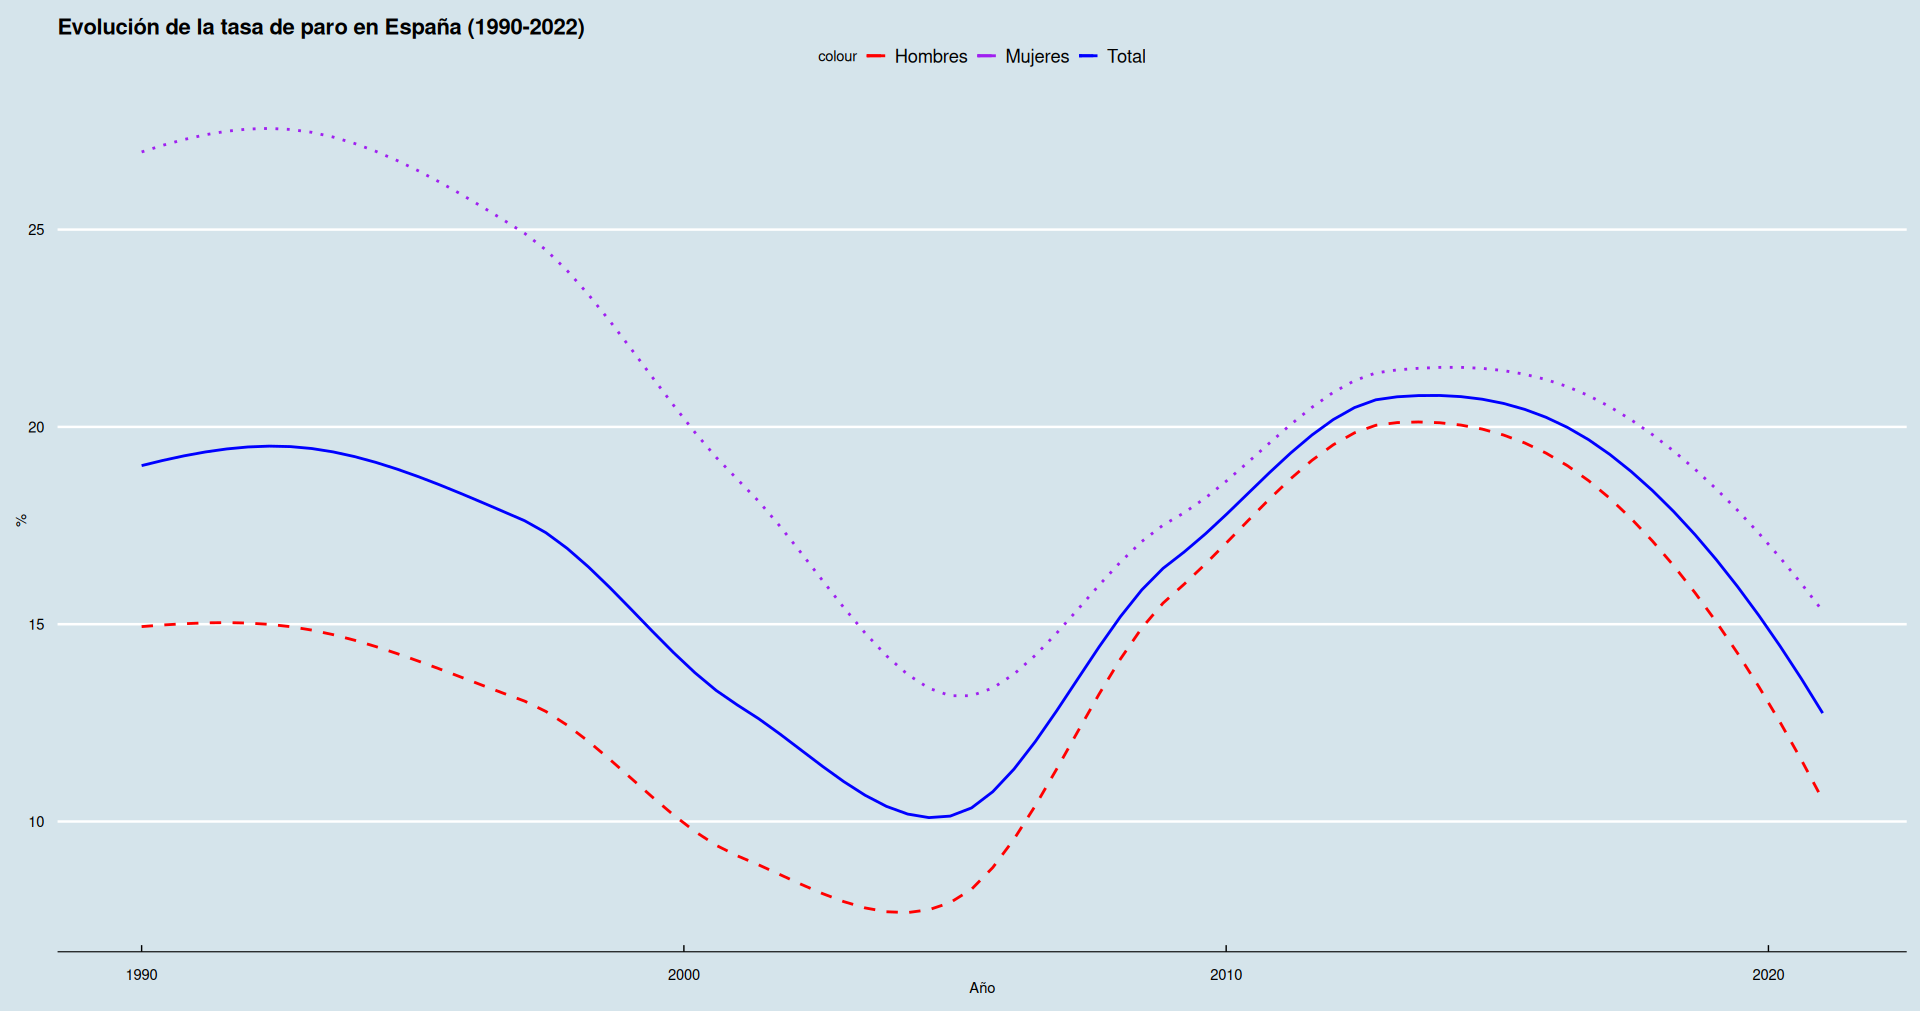
\includegraphics[scale=.32]{image/b3ej4e.png}
    \end{center}
    \vspace{.5cm}


Durante el periodo analizado de 1990 a 2021, se pueden destacar dos conclusiones relevantes sobre la evolución de la tasa de desempleo de las mujeres en España en comparación con la tasa de desempleo de los hombres y la tasa de desempleo total. En primer lugar, se observa una persistente brecha de género en el desempleo, donde la tasa de desempleo de las mujeres ha sido consistentemente más alta que la de los hombres a lo largo de los años. Aunque ambas tasas han experimentado fluctuaciones, las mujeres han enfrentado mayores dificultades en el mercado laboral, lo que señala la existencia de desigualdades estructurales y barreras que afectan su empleabilidad y acceso al trabajo. En segundo lugar, se observa una tendencia general de disminución en la tasa de desempleo tanto para hombres como para mujeres desde la crisis económica en 2008. Sin embargo, es importante destacar que la tasa de desempleo femenino se mantiene sistemáticamente por encima de la tasa de desempleo masculino. Estos hallazgos resaltan la necesidad de implementar políticas laborales y sociales que aborden las desigualdades de género en el mercado laboral español, promoviendo la igualdad de oportunidades y reduciendo las disparidades en la tasa de desempleo entre hombres y mujeres.\\\\

    \begin{center}
	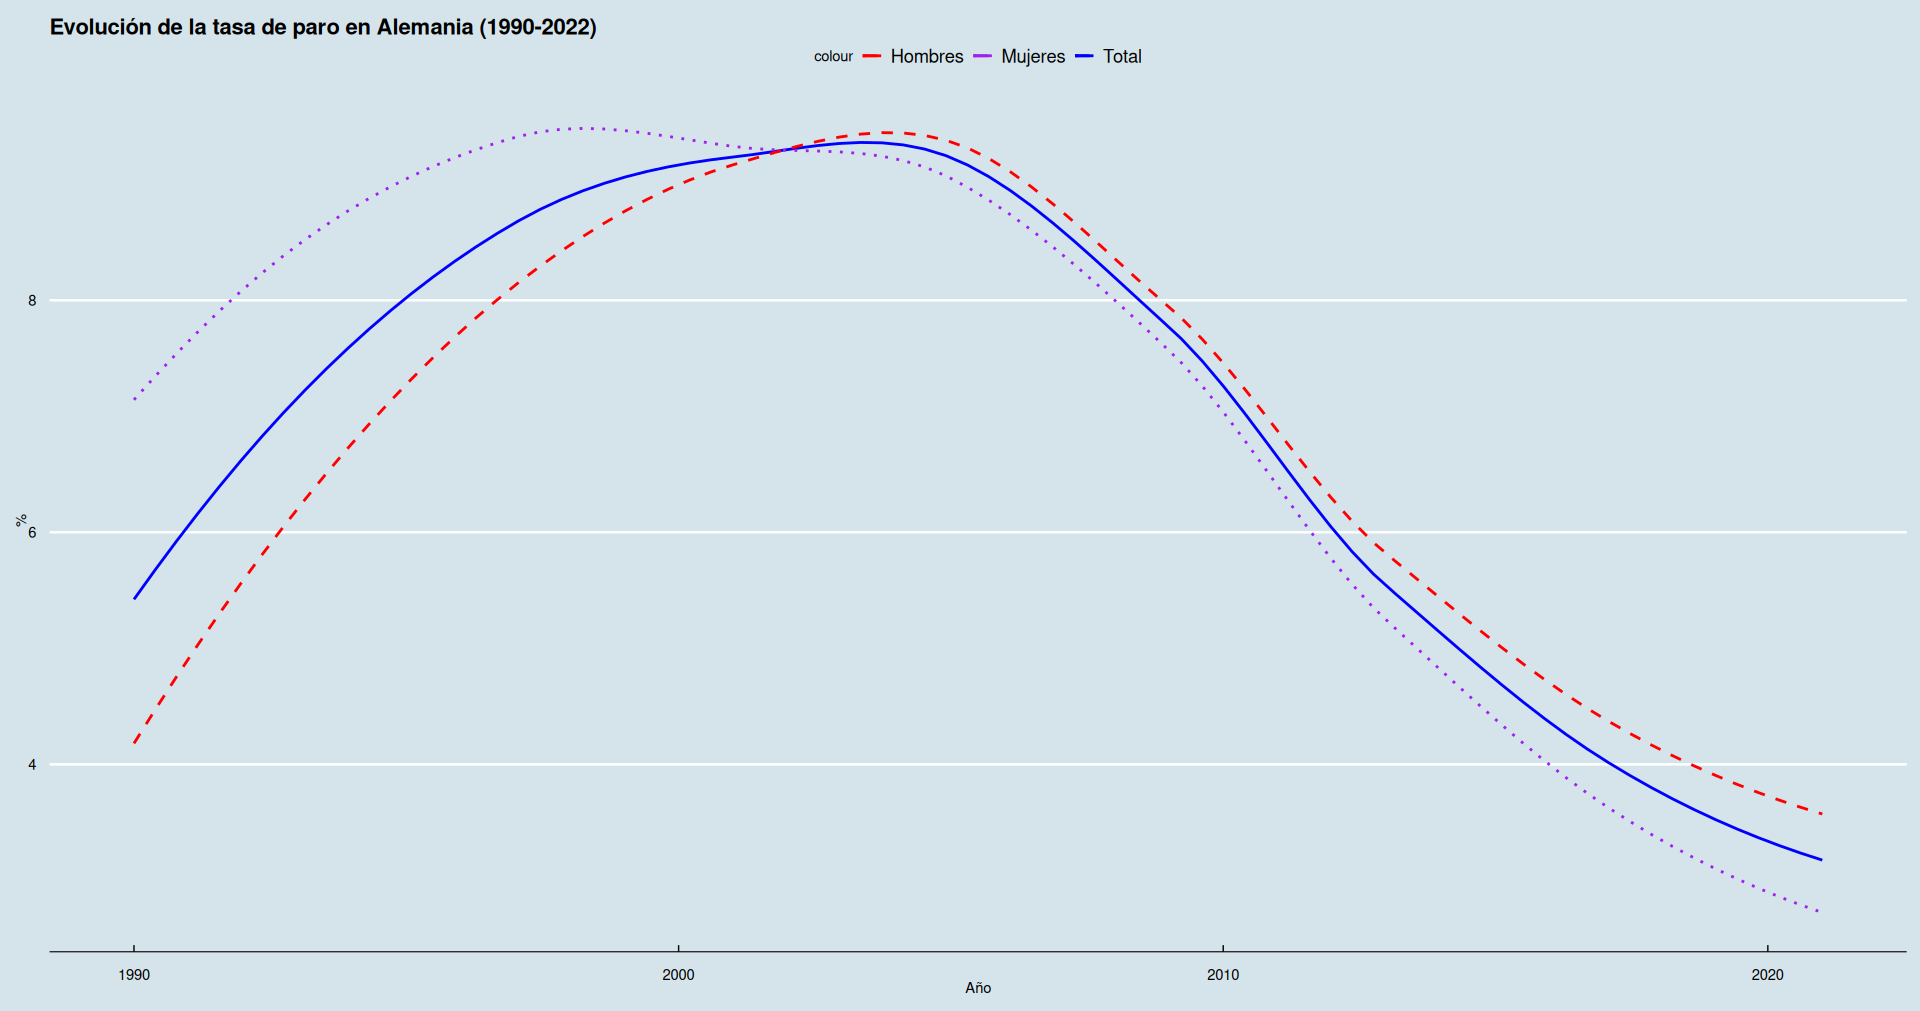
\includegraphics[scale=.32]{image/b3ej4a.png}
    \end{center}

    Durante el período analizado, desde 1990 hasta 2021, se puede observar una evolución en las tasas de desempleo en Alemania. Inicialmente, en la década de 1990, tanto hombres como mujeres experimentaron tasas de desempleo relativamente altas, siendo las mujeres ligeramente más afectadas. Sin embargo, a partir de mediados de la década de 2000, se aprecia una tendencia descendente en las tasas de desempleo tanto para hombres como para mujeres.\\\\

\textbf{Diagnostico del mercado de trabajo (4)}

    \begin{table}[htbp]
      \centering
      \begin{center}
      \end{center}
      \scalebox{0.5}{
	\begin{tabular}{r|*{3}{c}|*{3}{c}|*{3}{c}}
	\toprule
		&\multicolumn{3}{c|}{\textbf{España}} & \multicolumn{3}{c|}{\textbf{EU-27}} & \multicolumn{3}{c}{\textbf{OCDE}}\\
	   2021 (\%)&Total&Varones&Mujeres&Total&Varones&Mujeres&Total&Varones&Mujeres\\ 
	\midrule
	   \textbf{Tasa de actividad}&	58.5&63.6&53.7&74.5&78.7&69.6&&&\\
	   \textbf{Tasa de empleo}&	64.4&69.3&59.5&75.0&78.7&68.5&67.7&75.6&60.4\\
	   \textbf{Tasa de paro}&	14.8&13.1&16.7&7&6.7&7.4&6.2&6.0&6.4\\
	\bottomrule
	\end{tabular}%
	}
      \label{tab:addlabel}%
      \begin{center}
      \tiny Fuente: Celcdata.
      \end{center}
    \end{table}
    A pesar de esa favorable evolución de los últimos 10 años aproximadamente, aún España lejos de Europa en lo que a materia de desempleo se refiere. En la tabla se puede observar que la tasa de desempleo en España es más del doble que la de la Unión Europea y la OCDE.\\\\
    \vspace{.5cm}

    \begin{table}[htbp]
      \centering
      \begin{center}
      \end{center}
      \scalebox{0.5}{
	\begin{tabular}{r|*{3}{c}|*{3}{c}|*{3}{c}}
	\toprule
		&\multicolumn{3}{c|}{\textbf{Alemania}} & \multicolumn{3}{c|}{\textbf{EU-27}} & \multicolumn{3}{c}{\textbf{OCDE}}\\
	   2021 (\%)&Total&Varones&Mujeres&Total&Varones&Mujeres&Total&Varones&Mujeres\\ 
	\midrule
	   \textbf{Tasa de actividad}&	&&&74.5&78.7&69.6&&&\\
	   \textbf{Tasa de empleo}&	75.1&79.3&72.2&75.0&78.7&68.5&67.7&75.6&60.4\\
	   \textbf{Tasa de paro}&	3.6&3.9&3.2&7&6.7&7.4&6.2&6.0&6.4\\
	\bottomrule
	\end{tabular}%
	}
      \label{tab:addlabel}%
      \begin{center}
      \tiny Fuente: Celcdata.
      \end{center}
    \end{table}
    La tasa de paro tiene un valor del 3.6\% en Alemania, superior al del mismo indicador en la UE-27, que es del 7\%. En este caso, la tasa de paro de las mujeres es inferior a la de los hombres, lo que indica que las mujeres tienen más facilidad para encontrar empleo que los hombres.\\\\


    \textbf{Diagnostico del mercado de trabajo (5)}
